\documentclass[12pt, twoside]{book} % change to 'oneside' if not printing both sides

%\title{BE(Hons) 2017 thesis template}  % Edit if desired - used by "Overleaf", not currenty used by LaTeX

% The file "Preamble.tex" input here is required to set up the document - keep but edit if required

% =========================================================================
%                        Preamble
% No need to change anything unless you want to add a package.
% =========================================================================

% ESSENTIAL PACKAGES
% -------------------
\usepackage{graphicx}  % essential for inserting any figures
\usepackage[a4paper, left=35mm, right=25mm, top=50mm, bottom=30mm]{geometry}
\usepackage[absolute]{textpos} % required for the "textbox" command used in the title page. (Include option 'showboxes' if you want to see exact location)
   \setlength{\TPHorizModule}{1mm}
   \setlength{\TPVertModule}{1mm}% sets the units to be used for textpos


% SUGGESTED OPTIONAL PACKAGES
% ---------------------------
\usepackage{soul, todonotes}   % good for comments in drafts
\usepackage[authoryear]{natbib}  % recommended, especially for Harvard ref. styles
\usepackage{subfigure, longtable}
\usepackage[colorlinks=true, allcolors=blue]{hyperref}
   % soul & todonotes allow highlighting, comments etc (good for drafts)
   % subfigure allows subfigures (e.g. Fig 1(a) & (b))
   % longtable is handy if you include a nomenclature
   % natbib allows Harvard referencing (with appropriate bibliographystyle)
   % hyperref produces hyperlinks (sometimes clashes with other packages)

   % To include whole pdf pages (with example of use)
%\usepackage{pdfpages}
%\includepdf[pages={1-2}, angle=90, pagecommand={\thispagestyle{plain}}]{BoreBasePlateV2.pdf}

\renewcommand{\bibname}{References}   % Change "Bibliography" to "References"

% If you are using "Overleaf" include this so Overleaf knows what the main file is, otherwise delete this line, it is not used by LaTeX
\title{BE(Hons) 2017 thesis template}


\begin{document}

% =========================================================================
%                        Front matter 
%   Modify cover page, declaration, abstract, acknowledgements, Nomenclature
%   etc. as required. For draft purposes you can comment out some lines.
% =========================================================================
\frontmatter                % Don't delete this line

%      1.   Title page
%---------------------------
% May need to adjust dimensions: currently 120x55 @ (45,53) from top left of page (in mm)
\begin{textblock}{120}(45,53) % {width}(x,y) top-left rel to page top-left
\noindent\begin{minipage}[t][55mm][c]{\textwidth} 
\centering \Large  % change to '\large' if it doesn't fit
\vspace*{\fill}
{\bf UTas BE(Hons) Thesis Template:\\ with a title that takes up two lines or more}
\vfill
A.U. Thor, 123456 
\vfill
\large October 2017
\vspace*{\fill}
\end{minipage}
\end{textblock}

% Optional: University of Tasmania Logo
\begin{textblock}{120}(45,155)
\centering
\begin{figure}[h]
\centering
\includegraphics[width=0.75\linewidth]{UTAS-Logo-colour.eps}
\end{figure}
\vspace{2cm}
\Large
School of Engineering and ICT


\end{textblock}


% Footer of title page - edit only if you are doing BSc-BE(Hons)
% --------------------------------------------------------------
\begin{textblock}{150}(30,250)
\centering
\emph{This thesis is submitted in partial fulfilment of the requirements for the degree of
%Bachelor of Science and   %% uncomment this line if doing BSc-BE(Hons)
Bachelor of Engineering with Honours,
University of Tasmania.}
\end{textblock}



% suppress page numbering until declaration page
\pagenumbering{gobble}
\null\cleardoublepage
\pagenumbering{roman}

%      2.   Declaration
%---------------------------
\chapter{Declaration}

This Thesis to the best of my knowledge and belief contains no material published or unpublished that was written by another person, nor any material that infringes copyright, nor any material that has been accepted for a degree or diploma by University of Tasmania or any other institution, except by way of background information and where due acknowledgement is made in the text of the Thesis.

This Thesis is the result of my own investigations, except where otherwise stated. Other sources are acknowledged in the text giving explicit references. A list of references is appended.

% select one of the following paragraphs, modify if necessary

I hereby give consent for my Thesis to be available for photocopying, inter-library loan, electronic access to University of Tasmania staff and students via the University of Tasmania library, and for the title and summary to be made available to outside organisations, in accordance with the Copyright Act 1968.

%This thesis is not to be made available for loan or copying for [{\em insert period of time}] following the date of this statement. Following that time the thesis may be made available for loan and limited copying in accordance with the Copyright Act 1968.

   \bigskip
   \bigskip

Signed:

   \bigskip
   \bigskip

Dated: \hl{ 1st May 2018 }      % replace with an actual date if you don't want today's date
%      3.   Abstract
%---------------------------

\chapter{Abstract}

\hl{Insert your abstract here.}
%      4.   Acknowledgements
%---------------------------
\chapter{Acknowledgements}

People to thank are\ldots \hl{(insert your acknowledgements)}
\tableofcontents
\listoffigures   % optional
\listoftables    % optional
%      6.   Nomenclature (optional)
%---------------------------
\chapter{Nomenclature}
Notation below is reproduced from \citet{Goodfellow-et-al-2016}.

% From https://github.com/goodfeli/dlbook_notation/blob/master/notation.tex

\vspace{\notationgap}
% Need to use minipage to keep title of table on same page as table
\begin{minipage}{\textwidth}
	% This is a hack to put a little title over the table
	% We cannot use "\section*", etc., they appear in the table of contents.
	% tocdepth does not work on this chapter.
	\centerline{\bf Numbers and Arrays}
	\bgroup
	% The \arraystretch definition here increases the space between rows in the table,
	% so that \displaystyle math has more vertical space.
	\def\arraystretch{1.5}
	\begin{tabular}{cp{3.25in}}
		$\displaystyle a$ & A scalar (integer or real)\\
		$\displaystyle \va$ & A vector\\
		$\displaystyle \mA$ & A matrix\\
		$\displaystyle \tA$ & A tensor\\
		$\displaystyle \mI_n$ & Identity matrix with $n$ rows and $n$ columns\\
		$\displaystyle \mI$ & Identity matrix with dimensionality implied by context\\
		$\displaystyle \ve^{(i)}$ & Standard basis vector $[0,\dots,0,1,0,\dots,0]$ with a 1 at position $i$\\
		$\displaystyle \text{diag}(\va)$ & A square, diagonal matrix with diagonal entries given by $\va$\\
		$\displaystyle \ra$ & A scalar random variable\\
		$\displaystyle \rva$ & A vector-valued random variable\\
		$\displaystyle \rmA$ & A matrix-valued random variable\\
	\end{tabular}
	\egroup
	\index{Scalar}
	\index{Vector}
	\index{Matrix}
	\index{Tensor}
\end{minipage}

\vspace{\notationgap}
\begin{minipage}{\textwidth}
	\centerline{\bf Sets and Graphs}
	\bgroup
	\def\arraystretch{1.5}
	\begin{tabular}{cp{3.25in}}
		$\displaystyle \sA$ & A set\\
		$\displaystyle \R$ & The set of real numbers \\
		% NOTE: do not use \R^+, because it is ambiguous whether:
		% - It includes 0
		% - It includes only real numbers, or also infinity.
		% We usually do not include infinity, so we may explicitly write
		% [0, \infty) to include 0
		% (0, \infty) to not include 0
		$\displaystyle \{0, 1\}$ & The set containing 0 and 1 \\
		$\displaystyle \{0, 1, \dots, n \}$ & The set of all integers between $0$ and $n$\\
		$\displaystyle [a, b]$ & The real interval including $a$ and $b$\\
		$\displaystyle (a, b]$ & The real interval excluding $a$ but including $b$\\
		$\displaystyle \sA \backslash \sB$ & Set subtraction, i.e., the set containing the elements of $\sA$ that are not in $\sB$\\
		$\displaystyle \gG$ & A graph\\
		$\displaystyle \parents_\gG(\ervx_i)$ & The parents of $\ervx_i$ in $\gG$
	\end{tabular}
	\egroup
	\index{Scalar}
	\index{Vector}
	\index{Matrix}
	\index{Tensor}
	\index{Graph}
	\index{Set}
\end{minipage}

\vspace{\notationgap}
\begin{minipage}{\textwidth}
	\centerline{\bf Indexing}
	\bgroup
	\def\arraystretch{1.5}
	\begin{tabular}{cp{3.25in}}
		$\displaystyle \eva_i$ & Element $i$ of vector $\va$, with indexing starting at 1 \\
		$\displaystyle \eva_{-i}$ & All elements of vector $\va$ except for element $i$ \\
		$\displaystyle \emA_{i,j}$ & Element $i, j$ of matrix $\mA$ \\
		$\displaystyle \mA_{i, :}$ & Row $i$ of matrix $\mA$ \\
		$\displaystyle \mA_{:, i}$ & Column $i$ of matrix $\mA$ \\
		$\displaystyle \etA_{i, j, k}$ & Element $(i, j, k)$ of a 3-D tensor $\tA$\\
		$\displaystyle \tA_{:, :, i}$ & 2-D slice of a 3-D tensor\\
		$\displaystyle \erva_i$ & Element $i$ of the random vector $\rva$ \\
	\end{tabular}
	\egroup
\end{minipage}

\vspace{\notationgap}
\begin{minipage}{\textwidth}
	\centerline{\bf Linear Algebra Operations}
	\bgroup
	\def\arraystretch{1.5}
	\begin{tabular}{cp{3.25in}}
		$\displaystyle \mA^\top$ & Transpose of matrix $\mA$ \\
		$\displaystyle \mA^+$ & Moore-Penrose pseudoinverse of $\mA$\\
		$\displaystyle \mA \odot \mB $ & Element-wise (Hadamard) product of $\mA$ and $\mB$ \\
		% Wikipedia uses \circ for element-wise multiplication but this could be confused with function composition
		$\displaystyle \mathrm{det}(\mA)$ & Determinant of $\mA$ \\
	\end{tabular}
	\egroup
	\index{Transpose}
	\index{Element-wise product|see {Hadamard product}}
	\index{Hadamard product}
	\index{Determinant}
\end{minipage}

\vspace{\notationgap}
\begin{minipage}{\textwidth}
	\centerline{\bf Calculus}
	\bgroup
	\def\arraystretch{1.5}
	\begin{tabular}{cp{3.25in}}
		% NOTE: the [2ex] on the next line adds extra height to that row of the table.
		% Without that command, the fraction on the first line is too tall and collides
		% with the fraction on the second line.
		$\displaystyle\frac{d y} {d x}$ & Derivative of $y$ with respect to $x$\\ [2ex]
		$\displaystyle \frac{\partial y} {\partial x} $ & Partial derivative of $y$ with respect to $x$ \\
		$\displaystyle \nabla_\vx y $ & Gradient of $y$ with respect to $\vx$ \\
		$\displaystyle \nabla_\mX y $ & Matrix derivatives of $y$ with respect to $\mX$ \\
		$\displaystyle \nabla_\tX y $ & Tensor containing derivatives of $y$ with respect to $\tX$ \\
		$\displaystyle \frac{\partial f}{\partial \vx} $ & Jacobian matrix $\mJ \in \R^{m\times n}$ of $f: \R^n \rightarrow \R^m$\\
		$\displaystyle \nabla_\vx^2 f(\vx)\text{ or }\mH( f)(\vx)$ & The Hessian matrix of $f$ at input point $\vx$\\
		$\displaystyle \int f(\vx) d\vx $ & Definite integral over the entire domain of $\vx$ \\
		$\displaystyle \int_\sS f(\vx) d\vx$ & Definite integral with respect to $\vx$ over the set $\sS$ \\
	\end{tabular}
	\egroup
	\index{Derivative}
	\index{Integral}
	\index{Jacobian matrix}
	\index{Hessian matrix}
\end{minipage}

\vspace{\notationgap}
\begin{minipage}{\textwidth}
	\centerline{\bf Probability and Information Theory}
	\bgroup
	\def\arraystretch{1.5}
	\begin{tabular}{cp{3.25in}}
		$\displaystyle \ra \bot \rb$ & The random variables $\ra$ and $\rb$ are independent\\
		$\displaystyle \ra \bot \rb \mid \rc $ & They are conditionally independent given $\rc$\\
		$\displaystyle P(\ra)$ & A probability distribution over a discrete variable\\
		$\displaystyle p(\ra)$ & A probability distribution over a continuous variable, or over
		a variable whose type has not been specified\\
		$\displaystyle \ra \sim P$ & Random variable $\ra$ has distribution $P$\\% so thing on left of \sim should always be a random variable, with name beginning with \r
		$\displaystyle  \E_{\rx\sim P} [ f(x) ]\text{ or } \E f(x)$ & Expectation of $f(x)$ with respect to $P(\rx)$ \\
		$\displaystyle \Var(f(x)) $ &  Variance of $f(x)$ under $P(\rx)$ \\
		$\displaystyle \Cov(f(x),g(x)) $ & Covariance of $f(x)$ and $g(x)$ under $P(\rx)$\\
		$\displaystyle H(\rx) $ & Shannon entropy of the random variable $\rx$\\
		$\displaystyle \KL ( P \Vert Q ) $ & Kullback-Leibler divergence of P and Q \\
		$\displaystyle \mathcal{N} ( \vx ; \vmu , \mSigma)$ & Gaussian distribution %
		over $\vx$ with mean $\vmu$ and covariance $\mSigma$ \\
	\end{tabular}
	\egroup
	\index{Independence}
	\index{Conditional independence}
	\index{Variance}
	\index{Covariance}
	\index{Kullback-Leibler divergence}
	\index{Shannon entropy}
\end{minipage}

\vspace{\notationgap}
\begin{minipage}{\textwidth}
	\centerline{\bf Functions}
	\bgroup
	\def\arraystretch{1.5}
	\begin{tabular}{cp{3.25in}}
		$\displaystyle f: \sA \rightarrow \sB$ & The function $f$ with domain $\sA$ and range $\sB$\\
		$\displaystyle f \circ g $ & Composition of the functions $f$ and $g$ \\
		$\displaystyle f(\vx ; \vtheta) $ & A function of $\vx$ parametrized by $\vtheta$.
		(Sometimes we write $f(\vx)$ and omit the argument $\vtheta$ to lighten notation) \\
		$\displaystyle \log x$ & Natural logarithm of $x$ \\
		$\displaystyle \sigma(x)$ & Logistic sigmoid, $\displaystyle \frac{1} {1 + \exp(-x)}$ \\
		$\displaystyle \zeta(x)$ & Softplus, $\log(1 + \exp(x))$ \\
		$\displaystyle || \vx ||_p $ & $\normlp$ norm of $\vx$ \\
		$\displaystyle || \vx || $ & $\normltwo$ norm of $\vx$ \\
		$\displaystyle x^+$ & Positive part of $x$, i.e., $\max(0,x)$\\
		$\displaystyle \1_\mathrm{condition}$ & is 1 if the condition is true, 0 otherwise\\
	\end{tabular}
	\egroup
	\index{Sigmoid}
	\index{Softplus}
	\index{Norm}
\end{minipage}

Sometimes we use a function $f$ whose argument is a scalar but apply
it to a vector, matrix, or tensor: $f(\vx)$, $f(\mX)$, or $f(\tX)$.
This denotes the application of $f$ to the
array element-wise. For example, if $\tC = \sigma(\tX)$, then $\etC_{i,j,k} = \sigma(\etX_{i,j,k})$
for all valid values of $i$, $j$ and $k$.


\vspace{\notationgap}
\begin{minipage}{\textwidth}
	\centerline{\bf Datasets and Distributions}
	\bgroup
	\def\arraystretch{1.5}
	\begin{tabular}{cp{3.25in}}
		$\displaystyle \pdata$ & The data generating distribution\\
		$\displaystyle \ptrain$ & The empirical distribution defined by the training set\\
		$\displaystyle \sX$ & A set of training examples\\
		$\displaystyle \vx^{(i)}$ & The $i$-th example (input) from a dataset\\
		$\displaystyle y^{(i)}\text{ or }\vy^{(i)}$ & The target associated with $\vx^{(i)}$ for supervised learning\\
		$\displaystyle \mX$ & The $m \times n$ matrix with input example $\vx^{(i)}$ in row $\mX_{i,:}$\\
	\end{tabular}
	\egroup
\end{minipage}

\clearpage

% =========================================================================
%                        The main thesis body 
% Consider putting chapters etc. in separate files using \input{filename}
% =========================================================================
\mainmatter         % Don't delete this line
\chapter{Introduction}\todo[inline]{modify chapter headings as required}

\section{Background to the problem}

Normal `sentence case' is preferred for all headings, don't capitalise each word (e.g.~as above, not ``Background to the Problem").

\subsection{Brief Bib\TeX\ tips}

To illustrate the difference between \verb|\citet| and \verb|\citep|, and how to cite an honours thesis:
\begin{itemize}
  \item \citet{Smith} studied the problem of writing templates, but
  \item many examples of citing honours theses exist in the literature \citep{Smith}.
\end{itemize}
Refer to a standard as follows \citep{ISO3382-2}. With multiple authors make sure you separate each of the author's names with `and' \citep{BookExample}. Note the following features in this reference to \citet{vonKarman}:
\begin{itemize}
  \item multiple authors separated by `and' in the {\tt .bib} file,
  \item special character (\'a)
  \item compound surname needs to be contained in \{\}
  \item use of `DOI' reference (digital object identifier)  
\end{itemize}

More information can be found at \url{http://www.bibtex.org/} and some good examples at \url{https://verbosus.com//bibtex-style-examples.html}.

\subsection{Tables and figures}

Table~\ref{tab:demo} illustrates a simple table, while Figure~\ref{fig:demo} illustrates a figure with subfigures.



\begin{table}[htbp]
  \centering
  \begin{tabular}{ccl}
    \hline
    \textbf{Sample} & \textbf{Maximum recorded} &  \textbf{Failure location} \\
    \textbf{}		& \textbf{load (kN)}		&  \textbf{} \\
    \hline
    $C$    &  197.0  &  Top machined face     \\
    $U_1$  &  199.2  &  Above concrete        \\
    $U_2$  &  221.4  &  Top machined face     \\
    $W_1$  &  199.0  &  Middle machined face  \\
    $W_2$  &  197.0  &  Bottom machined face  \\
    \hline
    \end{tabular}
  \caption{A sample table.}
  \label{tab:demo}
\end{table}

\begin{figure}[htbp]
\centering
	\subfigure[Left subfigure.]{
        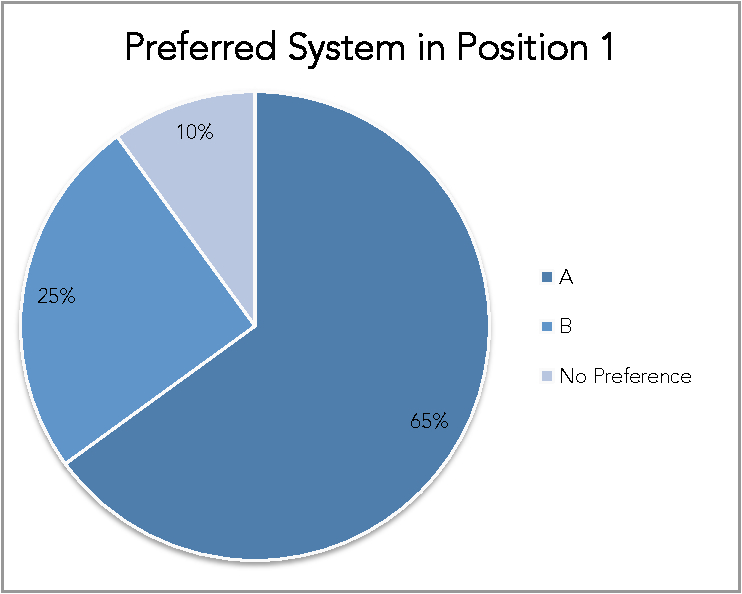
\includegraphics[width=.35\textwidth]{Pos1.pdf}
        \label{fig:Pos1}}
 \quad\quad
	\subfigure[Right subfigure.]{
        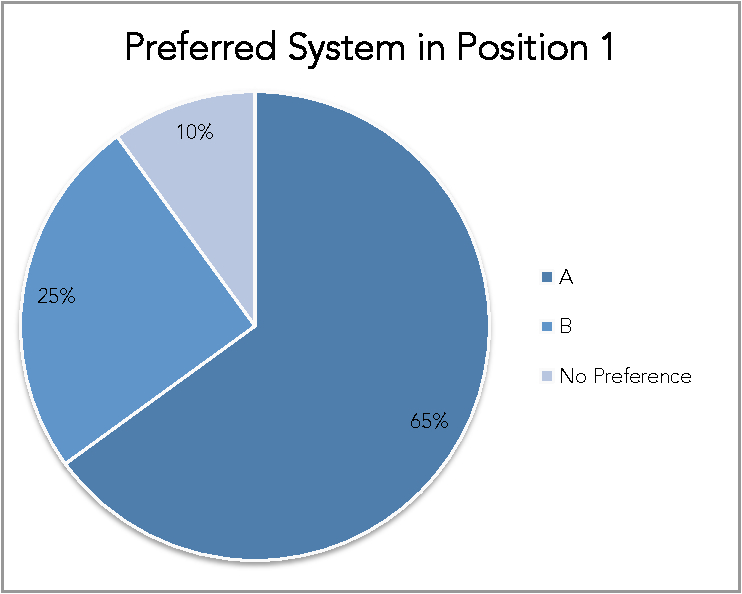
\includegraphics[width=.35\textwidth]{Pos1.pdf}
        \label{fig:Pos2}}
   \caption{A sample two part figure using the {\tt subfigure} package.}
  \label{fig:demo}
\end{figure}


\section{Problem statement}

\section{Project scope}

\chapter{Background theory}
   \section{Chapter intro}
   \section{Chapter body}
   \section{Chapter summary}

\chapter{Literature review}
   \section{Chapter intro}
   \section{Chapter body}
   \section{Chapter summary}

\chapter{Experimental method}
   \section{Chapter intro}
   \section{Chapter body}
   \section{Chapter summary}

\chapter{Results}
   \section{Chapter intro}
   \section{Chapter body}
   \section{Chapter summary}

\chapter{Discussion}
   \section{Chapter intro}
   \section{Chapter body}
   \section{Chapter summary}

\chapter{Conclusions and further work}
   \section{Summary of findings}
   \section{Limitations and recommendations}
   \section{Suggestions for further work}

% =========================================================================
%                        References/Bibliography
% Note that you must use a style that is compatible with the natbib package
% (e.g. plainnat or newapa) or remove "\usepackage{natbib}" from preamble.
% =========================================================================
\bibliographystyle{plainnat}   % choose a style here
\cleardoublepage \phantomsection \addcontentsline{toc}{chapter}{\bibname}  % This adds it to the table of contents with the right page numbering
\bibliography{ThesisTemplate}             % Your 'bib' file

% =========================================================================
%                        Appendices 
% =========================================================================
\appendix                 % This changes numbering from 1, 2 etc. to A, B etc.
\cleardoublepage          % these lines add it to the table of contents
\phantomsection
\addcontentsline{toc}{chapter}{Appendices}

%===================================
%       EDIT BELOW THIS LINE
%===================================

% The first appendix
\chapter{Extra stuff}

% The second appendix
\chapter{More extras}

% =========================================================================
%                        Back matter (if required, otherwise delete) 
% =========================================================================
%\backmatter

\end{document}